%\documentclass[10pt,dvips]{article}
\documentclass[10pt]{article}
\usepackage{../pplmanual}
\usepackage[pdftex]{graphicx}
%\usepackage[dvips]{graphicx}
%\usepackage[usenames,dvipsnames]{color}
%\usepackage[pdftex]{hyperref}
\usepackage{epsfig}
%%% Commonly Needed packages
\usepackage{graphicx,color,calc}
\usepackage{fancyvrb}
\usepackage{makeidx}
\usepackage{alltt}
\usepackage[linkbordercolor=(0 0 1),citebordercolor=(0 1 0)]{hyperref}
%%\usepackage{xspace} <- creates problems with other hyperlink packages like "html"

%%% Commands for uniform looks of C++, Charm++, and Projections
\newcommand{\CC}{C\hbox{++}}
\newcommand{\emCC}{C\hbox{\em++}}
\newcommand{\charmpp}{\textsc{Charm++}}
\newcommand{\charmc}{\texttt{charmc}}
\newcommand{\projections}{\textsc{Projections}}
\newcommand{\converse}{\textsc{Converse}}
\newcommand{\ampi}{\textsc{AMPI}}
\newcommand{\tempo}{\textsc{TeMPO}}
\newcommand{\irecv}{\textsl{iRecv}}
\newcommand{\sdag}{\textsl{Structured Dagger}}
\newcommand{\jade}{Jade}

%%% Commands to produce margin symbols
\newcommand{\new}{\marginpar{\fbox{\bf$\mathcal{NEW}$}}}
\newcommand{\important}{\marginpar{\fbox{\bf\Huge !}}}
\newcommand{\experimental}{\marginpar{\fbox{\bf\Huge $\beta$}}}

%%% Commands for manual elements
\newcommand{\zap}[1]{ }
\newcommand{\function}[1]{{\noindent{\textsf{#1}}\\}}
\newcommand{\cmd}[1]{{\noindent{\textsf{#1}}\\}}
\newcommand{\args}[1]{\hspace*{2em}{\texttt{#1}}\\}
\newcommand{\prototype}[1]{\vspace{0.2in}\index{#1}}
\newcommand{\param}[1]{{\texttt{#1}}}
\newcommand{\kw}[1]{{\textsf{#1}\index{#1}}}
\newcommand{\uw}[1]{{\textsl{#1}}}
\newcommand{\desc}[1]{\indent{#1}}
\newcommand{\note}[1]{(\textbf{Note:} #1)}
\newcommand{\term}[1]{{\bf #1}\index{#1}}

\makeindex


\ifpdf
\DeclareGraphicsExtensions{.jpg,.pdf,.mps,.png}
\else
\DeclareGraphicsExtensions{.eps}
\fi


\title{\projections{} Manual}
\version{2.1}
\credits{
By Mike DeNardo, Sid Cammeresi, Theckla Loucios, Orion Lawlor, Gengbin Zheng,
Chee Wai Lee, and Sindhura Bandhakavi
}

\begin{document}
\maketitle

\section{Introduction}

\projections{} is a parallel performance analysis/visualization tool
to help you understand and analyze what is happening in your parallel
(\charmpp{}) program. It is a post-mortem trace-based tool with
features that allow you to control the amount of information generated
and to a lesser degree the amount of perturbation the tracing
activities introduce into the application.

Performance analysis with \projections{} typically involves 3 phases:

\begin{itemize}
\item 
Instrumentation of user code (automated by default) and linking trace
generation modules. (see section \ref{sec::preparation})
\item
Generating trace data files. (see section \ref{sec::trace generation})
\item
Visualizing data and derived information (e.g. statistics); analyzing
possible performance problems (currently a manual process) of the
application. (see section \ref{sec::visualization})
\end{itemize}

\section{Preparing the \charmpp{} Application}
\label{sec::preparation}

The \charmpp{} runtime is automatically instrumented by default. This
means {\em most} users will not need to manually insert code into
their applications (see section \ref{sec::api}) in order to generate
trace data.

In the event that greater control over tracing activities
(e.g. dynamically turning instrumentation on and off) are desired,
\projections{} provides an API that allows users to insert code into
their applications for such purposes. Users may also register and
trace their own application-specific events (with limited support by
the visualization tool) via this API.

Please note that automatic instrumentation introduces the overhead of
an if-statement for each significant runtime event, even if no
performance analysis traces are desired.

Users who consider such an overhead to be unacceptable (e.g. for a
production application which requires the absolute best performance)
may recompile the \charmpp{} runtime with the {\tt -DCMK\_OPTIMIZE}
flag which removes the instrumentation stubs.

Otherwise, to enable the tracing of your application, users simply
need to link the appropriate trace data generation module(s) (also
referred to as {\em tracemode(s)}). (see section \ref{sec::trace modules})

\subsection{\projections{} API}
\label{sec::api}

\subsubsection{Selective Tracing}
\label{sec::selective tracing}

\charmpp{} allows user to start/stop tracing the execution at certain
points in time on the local processor. Users are advised to make these
calls on all processors and at well-defined points in the application.

Users may choose to have instrumentation turned off at first (by
command line option {\tt +traceoff} - see section \ref{sec::general options}) if some period of time in middle of the
application\'s execution is of interest to the user.

Alternatively, users may start the application with instrumentation
turned on (default) and turn off tracing for specific sections of the
application.

Again, users are advised to be consistent as the {\tt +traceoff}
runtime option applies to all processors in the application.

\begin{itemize}
\item
{\tt void traceBegin()}

Enables the runtime to trace events (including all user events) on the local processor where {\tt traceBegin} is called.

\item
{\tt void traceEnd()}

Prevents the runtime from tracing events (including all user events) on the local processor where {\tt traceEnd} is called.

\end{itemize}

\subsubsection{User Events}

\projections{} has a limited ability to visualize traceable user
specified events. You can make use of the following API calls to do
this. The general steps to do this are:

\begin{enumerate}
\item
Register an event with an identifying string and either specify or acquire
a globally unique event identifier.

\item
Use the event identifier to specify trace points in your code of interest to you.
\end{enumerate}

The functions available are as follows:

\begin{itemize}
\item
{\tt int traceRegisterUserEvent(char* EventDesc, int EventNum=-1) }

This function registers a user event by associating {\tt EventNum} to
{\tt EventDesc}. If {\tt EventNum} is not specified, a globally unique
event identifier is obtained from the runtime and returned.

{\tt EventNum} has to be the same on all processors. There are 3 ways
to ensure that, and correspondingly 3 ways to call the function:

\begin{enumerate}
\item
Call {\tt traceRegisterUserEvent} on node 0 in main::main without specifying
an event number, and store returned event number into a readonly variable.
\item
Call {\tt traceRegisterUserEvent} on all nodes without specifying an
event number. The returned value is the common event number that is
agreed on system-wide.
\item
Call {\tt traceRegisterUserEvent} and specify the event number on
processor 0. Doing this on other processors would have no
effect. Afterwards, the event number can be used in the following user
event calls.
\end{enumerate}

Eg. {\tt traceRegisterUserEvent("Time Step Begin", 10);}

Eg. {\tt eventID = traceRegisterUserEvent(``Time Step Begin'');}

\item
{\tt void traceUserEvent(int EventNum) }

This function works like a marker, indicating an occurrence of a
user-defined point event with the given {\tt EventNum}.

Eg. {\tt traceUserEvent(10);}

\item
{\tt void traceUserBracketEvent(int EventNum, double StartTime, double EndTime) }

This function records an event interval or activity identified by {\tt
EventNum} that lasts the period of time between {\tt StartTime} and
{\tt EndTime}. Both {\tt StartTime} and {\tt EndTime} can be obtained
from function call {\tt CmiWallTimer()} in seconds.

Eg.
\begin{verbatim}
   traceRegisterUserEvent("Critical Code", 20);
   double critStart;  // times of start
   critStart = CmiWallTimer();
   // do the critical code
   traceUserBracketEvent(20, critStart,CmiWallTimer());
\end{verbatim}

\end{itemize}

\subsection{Tracemodes}
\label{sec::trace modules}

Currently there are 2 tracemodes available. Zero or more tracemodes
may be specified at link-time. When no tracemodes are specified, no
trace data is generated.

\subsubsection{Projections mode}

Link time option: {\tt -tracemode projections}

This tracemode generates detailed log files that contain information
about all \charmpp{} events like entry method calls and message
packing during the execution of the program.  The data will be used by
\projections{} in visualization and analysis.

This tracemode generates a single symbol table file and $p$ ASCII log
files for $p$ processors. The names of the log files will be
NAME.\#.log where NAME is the name of your executable and \# is the
processor \#. The name of the symbol table file is NAME.sts where NAME
is the name of your executable.

This is the main source of data expected by the performance
visualizer. Certain tools like timeline will not work without the
detailed data from this tracemode. Refer to \ref{apx::file
formats} for more information about the format of the files generated
by this tracemode.

See section \ref{sec::projections runtime options} for application runtime
options available to this tracemode for generating trace data.

\subsubsection{Summary mode}

Compile option: {\tt -tracemode summary}

In this tracemode, execution time across all entry points for each
processor is partitioned into a fixed number of equally sized
time-interval bins. These bins are globally resized whenever they are
all filled in order to accomodate longer execution times while keeping
the amount of space used constant.

Additional data like the total number of calls made to each entry
point is summarised within each processor.

This tracemode generates a single symbol table file and $p$ ASCII
summary files for $p$ processors. The names of the summary files will
be NAME.\#.sum where NAME is the name of your executable and \# is the
processor \#. The name of the symbol table file is NAME.sum.sts where NAME
is the name of your executable.

This tracemode can be used to control the amount of output generated
in a run. It is typically used in scenarios where a quick look at the
overall utilization graph of the application is desired to identify
smaller regions of time for more detailed study. Attempting to
generate the same graph using the detailed logs of the prior tracemode
may be unnecessarily time consuming or impossible.

See section \ref{sec::summary runtime options} for application runtime
options available to this tracemode for generating trace data.

\section{Generating trace data}
\label{sec::trace generation}

A set of runtime options are available to you depending on which {\em
tracemode(s)} you have specified at link time. These are used to
control various aspects of trace file output.

The appropriate files (see preceeding descriptions of available
tracemodes) are generated automatically when the application is run.

\subsection{General runtime options}
\label{sec::general options}

The following is a list of runtime options available with the same
semantics for all tracemodes:

\begin{itemize}
\item
{\tt +traceroot DIR}: place all generated files in DIR.
\item
{\tt +traceoff}:      trace generation is turned off when the application is started. The user is expected to insert code to turn tracing on at some point in the run.
\end{itemize}

\subsection{Projections tracemode runtime options}
\label{sec::projections runtime options}

The following is a list of runtime options available under this tracemode:

\begin{itemize}
\item
{\tt +logsize NUM}:   keep only NUM log entries in the memory of each processor. The logs are emptied and flushed to disk when filled.
\item
{\tt +binary-trace}:  generate projections log in binary form.
\item
{\tt +gz-trace}:      generated gzip (if available) compressed log files.
\end{itemize}

\subsection{Summary tracemode runtime options}
\label{sec::summary runtime options}

The following is a list of runtime options available under this tracemode:

\begin{itemize}
\item
{\tt +bincount NUM}:   use NUM time-interval bins. The bins are resized and compacted when filled.
\item
{\tt +binsize TIME}:   sets the initial time quantum each bin represents.
\item
{\tt +version}:        set summary version to generate.
\end{itemize}

\section{The \projections{} Performance Visualization Tool}
\label{sec::visualization}

\projections{} comes pre-built with the \charmpp{} source release. It can
be located at \\
{\tt CHARM\_LOCATION/tools/projections} which will henceforth be refered 
to as {\tt PROJECTIONS\_LOCATION}.

\subsection{Building \projections{}}

To rebuild \projections{} (optional) from the source:

\begin{enumerate}
\item[1)]
   Make sure the JDK commands ``java'', ``javac'' and ``jar''
   are in your path
\item[2)]
   From {\tt PROJECTIONS\_LOCATION/}, type ``make''
\item[3)]
   The following files are placed in `bin':

      {\tt projections}           : Starts projections, for UNIX machines

      {\tt projections.bat}       : Starts projections, for Windows machines

      {\tt projections.jar}       : archive of all the java and image files
\end{enumerate}

\subsection{Visualization and Analysis using \projections{}}

\subsubsection{Starting Up}

From any location, type: \\
{\tt > PROJECTIONS\_LOCATION/bin/projections [NAME.sts]} \\
where {\tt PROJECTIONS\_LOCATION} is the path to the main projections
directory.

Supplying the optional {\tt NAME.sts} file in the command line will
cause projections to load data from the file at startup. This shortcut
saves time selecting the desired dataset via the GUI's file dialog.

\begin{figure}[hbt]
\center
%\epsfig{figure=fig/front-with-summary.eps,height=4in}
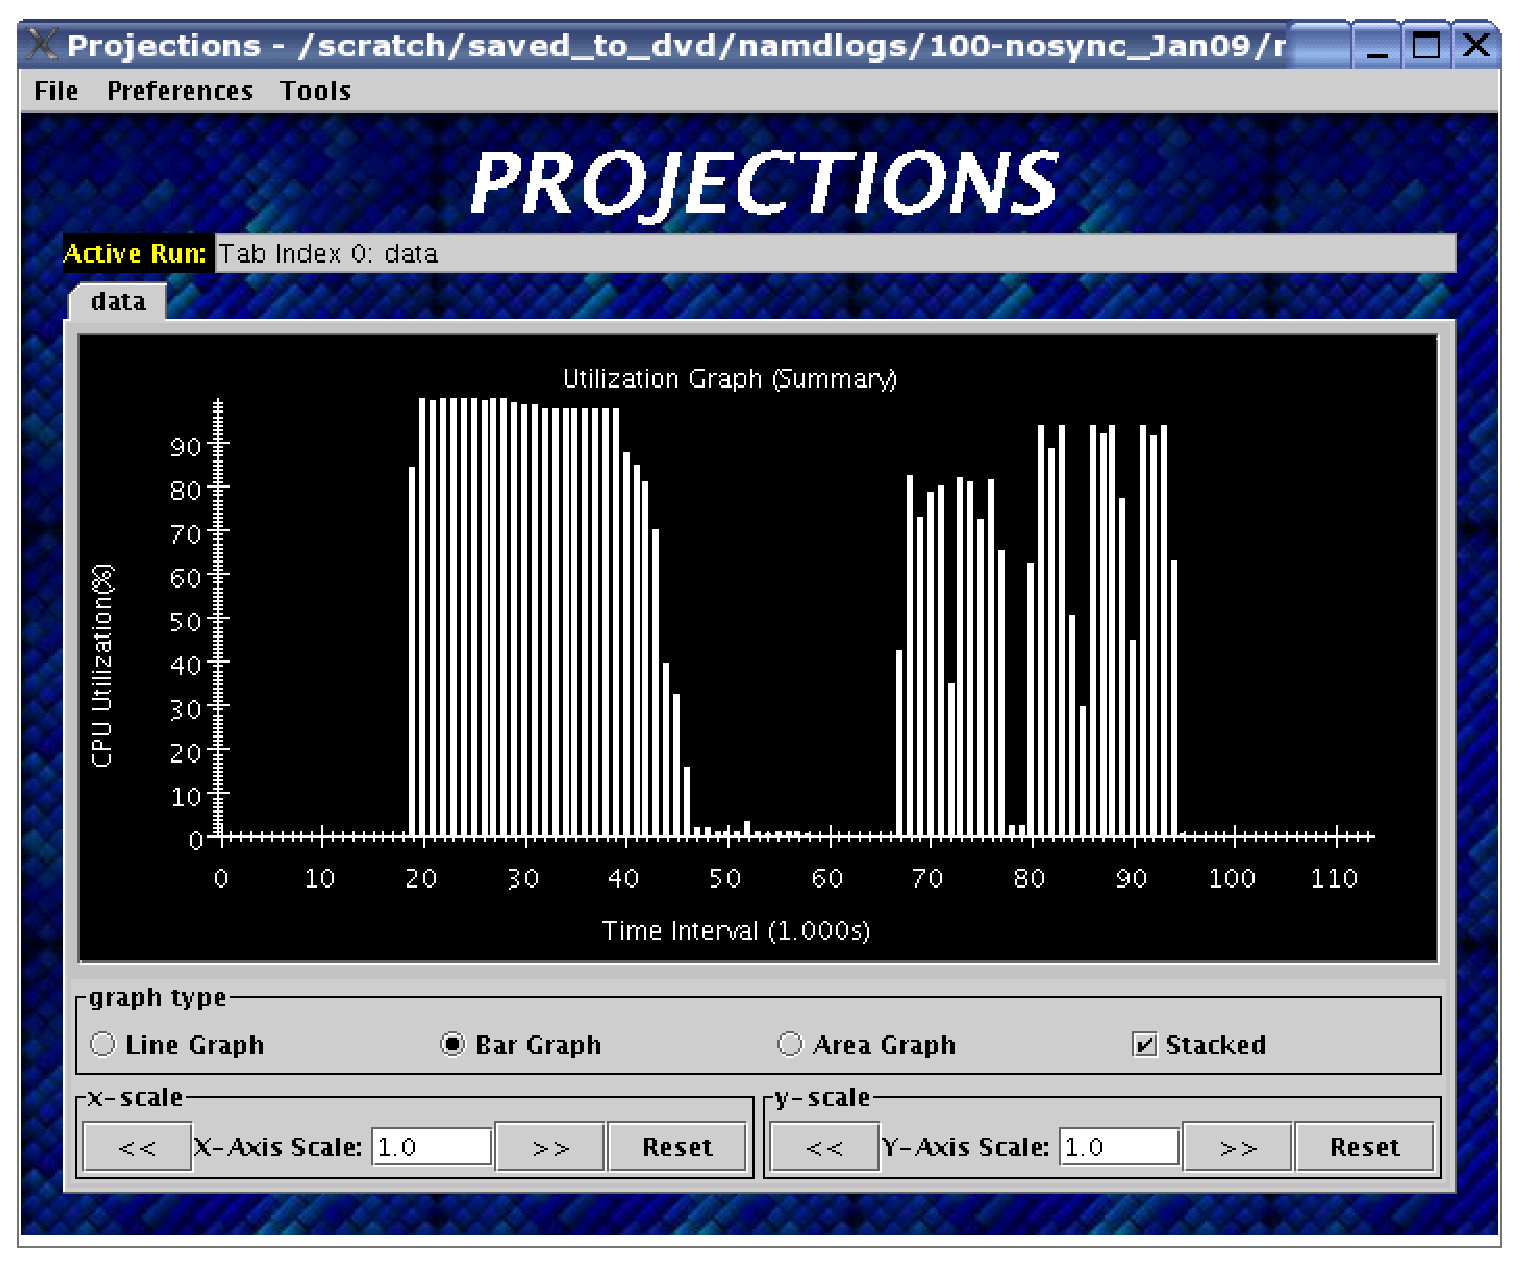
\includegraphics[width=4.0in]{fig/front-with-summary}
\caption{\projections{} main window}
\label{mainwindow}
\end{figure}


When \projections{} is started, it will display a main window as shown
in figure \ref{mainwindow}. If summary (.sum) files are available in
the set of data, a low-resolution utilization graph will be displayed
as shown. Otherwise, the main window shows a blank screen.

\subsubsection{Loading a Set of Log Data}

If you had not specified a {\tt NAME.sts} file in the command line
when starting \projections{}, you can choose to load a dataset via
the menu sequence File$->$Open File(s).

This brings up a dialog box that allows you to select the location of
the dataset you wish to study. Navigate to the directory containing
your data and select the .sts file.  Click on 'Open'.  If you have
selected a valid file, \projections{} will load in some preliminary
data from the files and then activate the rest of the options under
the menu item Tools.

\subsubsection{Available Tools}

The following tools and views become available to you after a dataset
has been loaded (with the exception of Multirun Analysis) and may be
accessed via the menu item Tools:

\begin{itemize}
\item 
The {\bf Graphs} view is where you can analyze your data by breaking it
into any number of intervals and look at what goes on in each of those
intervals.
\item
The {\bf Timelines} view lets you look at what a specific processor is
doing at each moment of the program. It is the most detailed view of a
parallel application \projections{} offers (and correspondingly, the
most resource-hungry).
\item
The {\bf Usage Profile} view lets you see percentage-wise what entry
methods each processor spends its time on during a specified time range.
It is particularly useful for identifying load imbalance and the probable
offending entry method.
\item
The {\bf Communication Histogram} view COMMUNICATION HISTOGRAM DESCRIPTION
\item
The {\bf Log File Viewer} provides a human-readable, verbose
interpretation of a log file's entries.
\item
The {\bf Histograms} view HISTOGRAM SUMMARY DESCRIPTION.
\item
The {\bf Overview} view gives user an overview of the utilization of
all processors during the execution. It is an extremely useful initial
tool to begin your performance analysis efforts with as it provides an
overall picture of application performance while being very
light-weight at the same time.
\item
The {\bf Animation} view animates the processor usage over a specified
range of time and a specified interval size.
\item
The {\bf Time Profile Graph} view TIME PROFILE SUMMARY DESCRIPTION
\item
The {\bf Multirun Analysis} view is still a work in progress. THE INTENDED
YADA YADA YADA ...
\end{itemize}

\subsubsection{Graphs}
\label{sec::graph view}
The Graphs window is where you can analyze your data by breaking it
into any number of intervals and look at what goes on in each of those
intervals.

When the Graph Window first appears, a dialog box will also appear,
asking you what interval settings you want to use.  It will show you
the total amount of time your program run took (in microseconds) and
ask you to enter either the interval size you want or the number of
intervals you want.  Entering a number in either box will recalculate
the other number, so you will know both items. Click on 'OK' when you
are satisifed with your choice.  Your data will then be analyzed.

The amount of time to analyze your data depends on several factors,
including the number of processors, number of entries, and number of
intervals you have selected.  Although a progress meter has not been
implemented at this time, you can look at the console window to see
which log file is being analyzed.  Even for large amounts of data,
this step should not take more than a few minutes, though.

\begin{figure}[hbt]
\center
%\epsfig{figure=fig/graph.eps,height=4.3in}
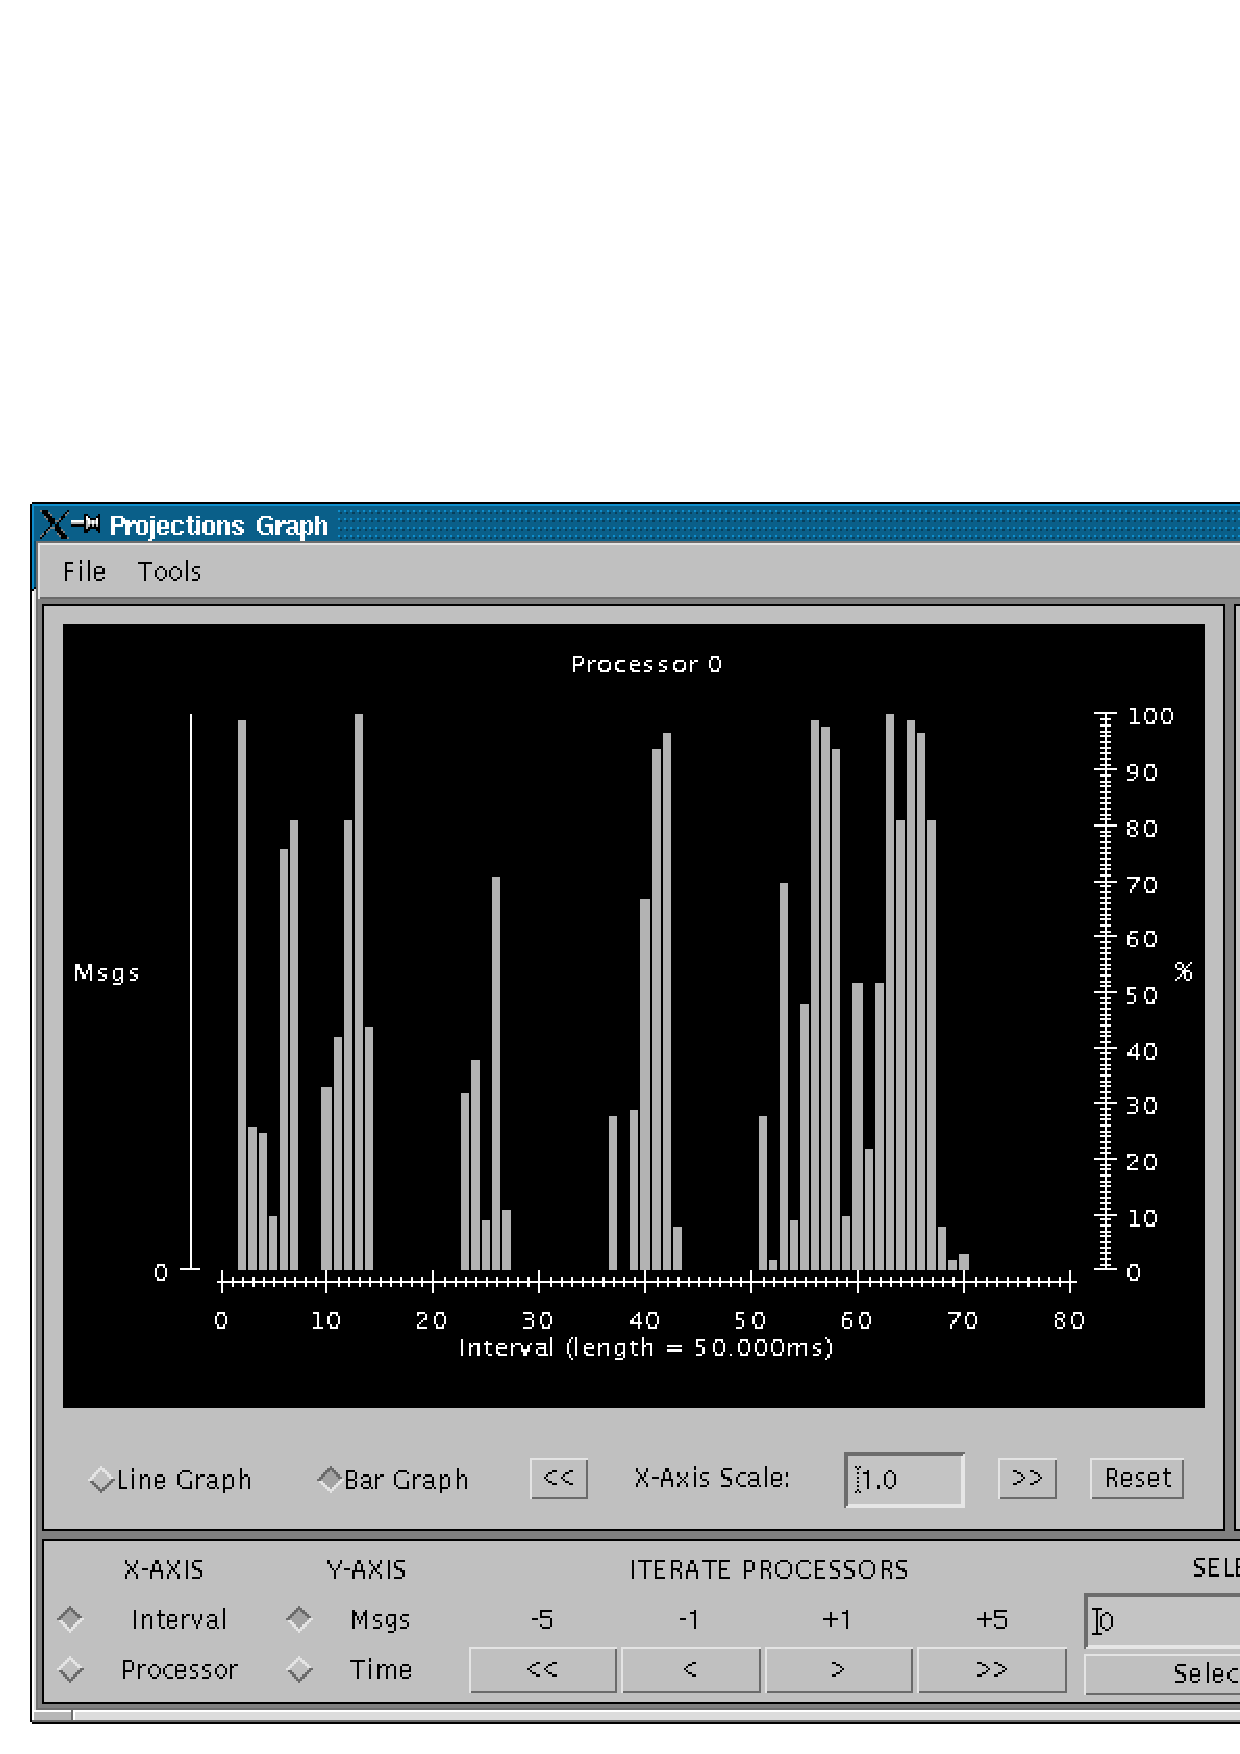
\includegraphics[width=4.3in]{fig/graph}
\caption{Graph module}
\label{graph}
\end{figure}



The Graph Window has 3 components in its display:
\begin{enumerate}
\item[1)]
Display Panel:
   \begin{itemize}
   \item[-]
   Largest Component in top/left corner
   \item[-]
   Displays title, graph, and axes
   \item[-]
   Allows you to toggle display between a line graph and a bar graph
   \item[-]
   Allows you to scale the graph along the X-axis.  You can either
   enter a scale value $>=$ 1.0 in the text box, or you can use the
   $<<$ and $>>$ buttons to increment/decrement the scale by .25.
   Clicking on Reset sets the scale back to 1.0.  When the scale is
   greater than 1.0, a scrollbar will appear along the bottom of the
   graph to let you scroll back and forth.
   \end{itemize}
\item[2)]
Legend Panel:
   \begin{itemize}
   \item[-]
   Top right side of the display
   \item[-]
   Shows what is currently being displayed on the graph and what color it
   is.
   \item[-]
   Click on the 'Select Display Items' button to bring up a window to
   add/remove items from the graph and to change the colors of the items.
      \begin{itemize}
      \item[*]
      The Select Display Items window shows a list of items that you
      can display on the graph.  There are 3 main sections: System
      Usage, System Msgs, and User Entries The System Usage and System
      Msgs are the same for all programs.  The User Entries section
      has program-specific items in it.
      \item[*]
      Click on the checkbox next to an item to have it displayed on the
      graph.
      \item[*]
      Click on the colorbox next to an item to modify its color.
      \item[*]
      Click on 'Select All' to choose all of the items
      \item[*]
      Click on 'Clear All' to remove all of the items
      \item[*]
      Click on 'Apply' to apply you choices/changes to the graph
      \item[*]
      Click on 'Close' to exit
      \end{itemize}
   \end{itemize}
\item[3)]
Control Panel:
   \begin{itemize}
   \item[-]
   Bottom of the display
   \item[-]
   Allows you to toggle what is displayed on the X-axis.  You can either
   have the x-axis display the data by interval or by processor.
   \item[-]
   Allows you to toggle what is displayed on the Y-axis.  You can
   either have the y-axis display the data by the number of msgs sent
   or by the amount of time taken.
   \item[-]
   Allows you to change what data is being displayed by iterating
   through the selections.  If you have selected an x-axis type of
   'interval', that means you are looking at what goes on in each
   interval for a specific processor.  Clicking on the $<<, <, >, >>$
   buttons will change the processor you are looking at by either -5,
   -1, +1, or +5.  Conversely, if you have an x-axis of 'processor',
   then the iterate buttons will change the value of the interval that
   you are looking at for each processor.
   \item[-]
   Allows you to indicate which intervals/processors you want to
   examine.  Instead of just looking at one processor or one interval,
   the box and buttons on the right side of this panel let you choose
   any number or processors/intervals to look at.  Just enter the
   number(s) in the box.  If you want to look at multiple items,
   separate them with commas.  If your selections include a range of
   items, you can separate those with a dash.

   ex: Want to see processors 1,3,5,7:  Enter 1,3,5,7

   ex: Want to see processors 1,2,3,4:  Enter 1-4

   ex: Want to see processors 1,2,3,7:  Enter 1-3,7

   Clicking on 'Apply' updates the graph with your choices. Clicking
   on 'Select All' chooses the entire range.  When you select more
   than one set of data to display, the graph will show the TOTAL
   amount of the data for all of those items, EXCEPT for the processor
   usage, which shows the average amount.
   \end{itemize}
\end{enumerate}

\subsubsection{Timelines}
\label{sec::timeline view}
The Timeline window lets you look at what a specific processor is
doing at each moment of the program.

\begin{figure}[htb]
\center
%\epsfig{figure=fig/timeline.eps,height=3.8in}
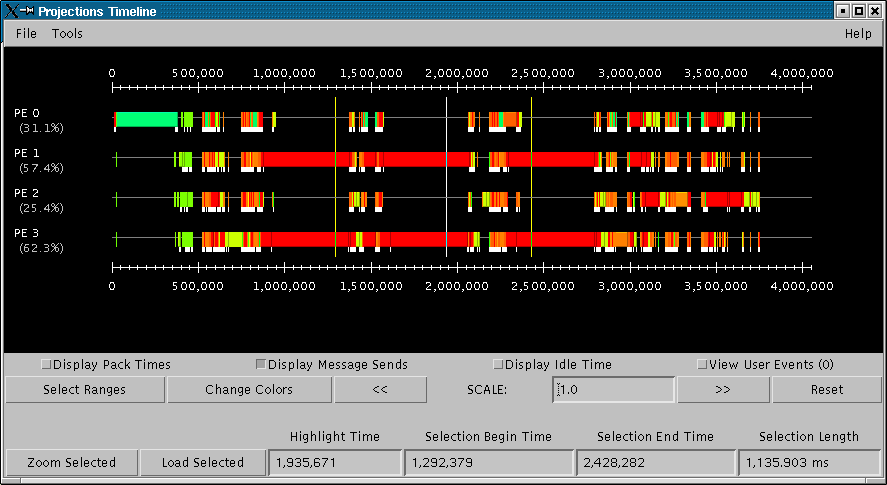
\includegraphics[width=3.8in]{fig/timeline}
\caption{Timeline module}
\label{timeline}
\end{figure}

When the Timeline window first appears, a dialog box appears along
with it. The box asks for the following information:

\begin{itemize}
\item[-]
Processor(s): Choose which processor(s) you want to see a timeline
for. To enter multiple values, separate them with a comma or a dash
(for ranges). (See the Graphs section \ref{sec::graph view} for 
examples)
\item[-]
Begin Time  : Choose what time you want your timeline to start at.
\item[-]
End Time    : Choose what time you want your timeline to end at.
\item[-]
Length      : Choose the length of your timeline.
\end{itemize}

The dialog box tells you what the valid processor choices are as well as what
the valid time ranges are.

Instead of entering a BeginTime, you can have the dialog box choose a
BeginTime for you based on the occurrence of a specific entry.  To do
this, you go to the bottom portion of the dialog box and select an
entry to find an occurrence of.  Then, you choose the processor you
want to find an occurrence on, and which occurrence you want to find
(N). Click on 'Search for Begin Time'.  The dialog box will display a
message telling you if your occurrence was found and when it was
found. If valid, the time is automatically entered as the begin time.

When you are satisifed with your time and processor ranges, click on
'OK'.  \projections{} will then get the Timeline data for you.  The
time for this step depends on the number of items in your time range
and the number of processors you have chosen.

The Timeline Window consists of two parts:
\begin{enumerate}
\item[1)]
Display Panel:

This is where the timelines are displayed and is the largest portion
of the window.  The time axes are displayed at the top and the bottom
of the panel, and the units are microseconds.  The left side of the
panel shows the processor labels.  Underneath each label is a
percentage telling you what amount of the total time in your timeline
was actually spent working on this program.

The timeline itself consists of colored bars for each work item.
Placing the cursor over one of these bars will bring up a pop-up
window telling you the name of that item, the begin time, the end
time, and the total time.  It will also tell you what amount of time
was spent packing, how many messages were created during this work
item, and which processor created this item. 

User events are also displayed as thin lines or bars above ordinary
event bars in the display area.

Display Panel features include:
   \begin{itemize}
   \item[-] 
   Detailed Information Pop-up - If you left-click on an item, a
   window will appear telling you similar information to the pop-up
   window.  This window will also list all of the messages created
   during this work item, and it will tell you what time they were
   sent at and to which entry.
   \item[-]
   Message Source Lines - If you right-click on an item, a white line
   will be drawn from the beginning of that item to the source of the
   message send that created the item. This line can only be drawn if
   the source lies within the loaded time range. Additionally, if the
   processor on which the source lies is not loaded, \projections{}
   will automatically load it into the timeline.
   \end{itemize}

\item[2)]
Control Panel:

It's located at the bottom of the window. Its components are described
as follows.

Checkboxes:
   \begin{itemize}
   \item[-]
   Display Pack Times - Lets you toggle display of Time spent packing
   \item[-] 
   Display Message Creations - Lets you toggle display of message
   creations. These are represented by little vertical lines at the
   time a message was created.
   \item[-]
   Display Idle Time - Lets you toggle display of idle time.
   \item[-]
   View User Event - Checking this box will bring up a new window
   showing the string description, begin time, end time and duration
   of all user events on each processor.  Especially, the user event
   caught by function {\tt traceUserEvent} has a duration of 0.

   \begin{figure}[htb]
   \center
%\epsfig{figure=fig/userevent.eps,height=1.5in}
   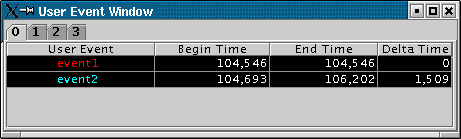
\includegraphics[height=1.5in]{fig/userevent}
   \caption{User Event Window}
   \label{userevent}
   \end{figure}

   \end{itemize}

Buttons:
   \begin{itemize}
   \item[-]
   Select Ranges - Brings up the initial dialog box.
   \item[-]
   Change Colors - Lets you change colors for the work items.
   \item[-]
   Scale - Enter a scale $>=$ 1.0 in the box, or click on the $<<$ and
   $>>$ buttons to adjust the scale by 0.25 increments.  Click on
   Reset to set the scale back to 1.0
   \end{itemize}
\end{enumerate}

An additional feature of timeline is a quick interface to zoom into an
area of interest, described below:

To determine the exact time of any event on the timeline, move your
mouse along either the top or bottom axis and a white vertical
highlight line will show where your cursor is along the timeline. The
``Highlight Time'' box on the bottom of the Timeline window will show
the exact time based on the location of your cursor.

To select an area, click on the axis to define the start of the area
and drag the mouse to the end of the area to be defined.  Two yellow
vertical lines will bracket the area of interest.  The exact times of
the selected area will be shown in the ``Selection Start Time'' text
area and the ``Selection End Time'' text area.  The difference between
these times is shown in ms in the ``Selected Length'' text area.  Thus,
this feature can be used to measure the time between two events of
interest across processors, and is an easy way to measure the time of
an entry point (instead of getting the ``Tool Tip'' balloon by putting
the cursor in the entry point.

To then zoom into the selected area via this interface, click on
either the ``Zoom Selected'' or the ``Load Selected'' buttons.  The
difference between these two buttons is that the "Load Selected" zooms
into the selected area and discards any events that are outside the
time range.  This is more efficient than ``Zoom Selected'' as the
latter draws all the events on a virtual canvas and then zooms into
the canvas. The disadvantage of using ``Load Selected'' is that it
becomes impossible to zoom back out without having to re-specify the
time range via the ``Select Ranges'' button.

\subsubsection{Usage Profile}

The Usage Profile window lets you see percentage-wise what each processor
spends its time on during a specified period.

When the window first comes up, a dialog box appears asking for the
processor(s) you want to look at as well as the time range you want to
look at.  This is similar to the dialog for the Timelines.

\begin{figure}[htb]
\center
%\epsfig{figure=fig/usageprofile.eps,height=4in}
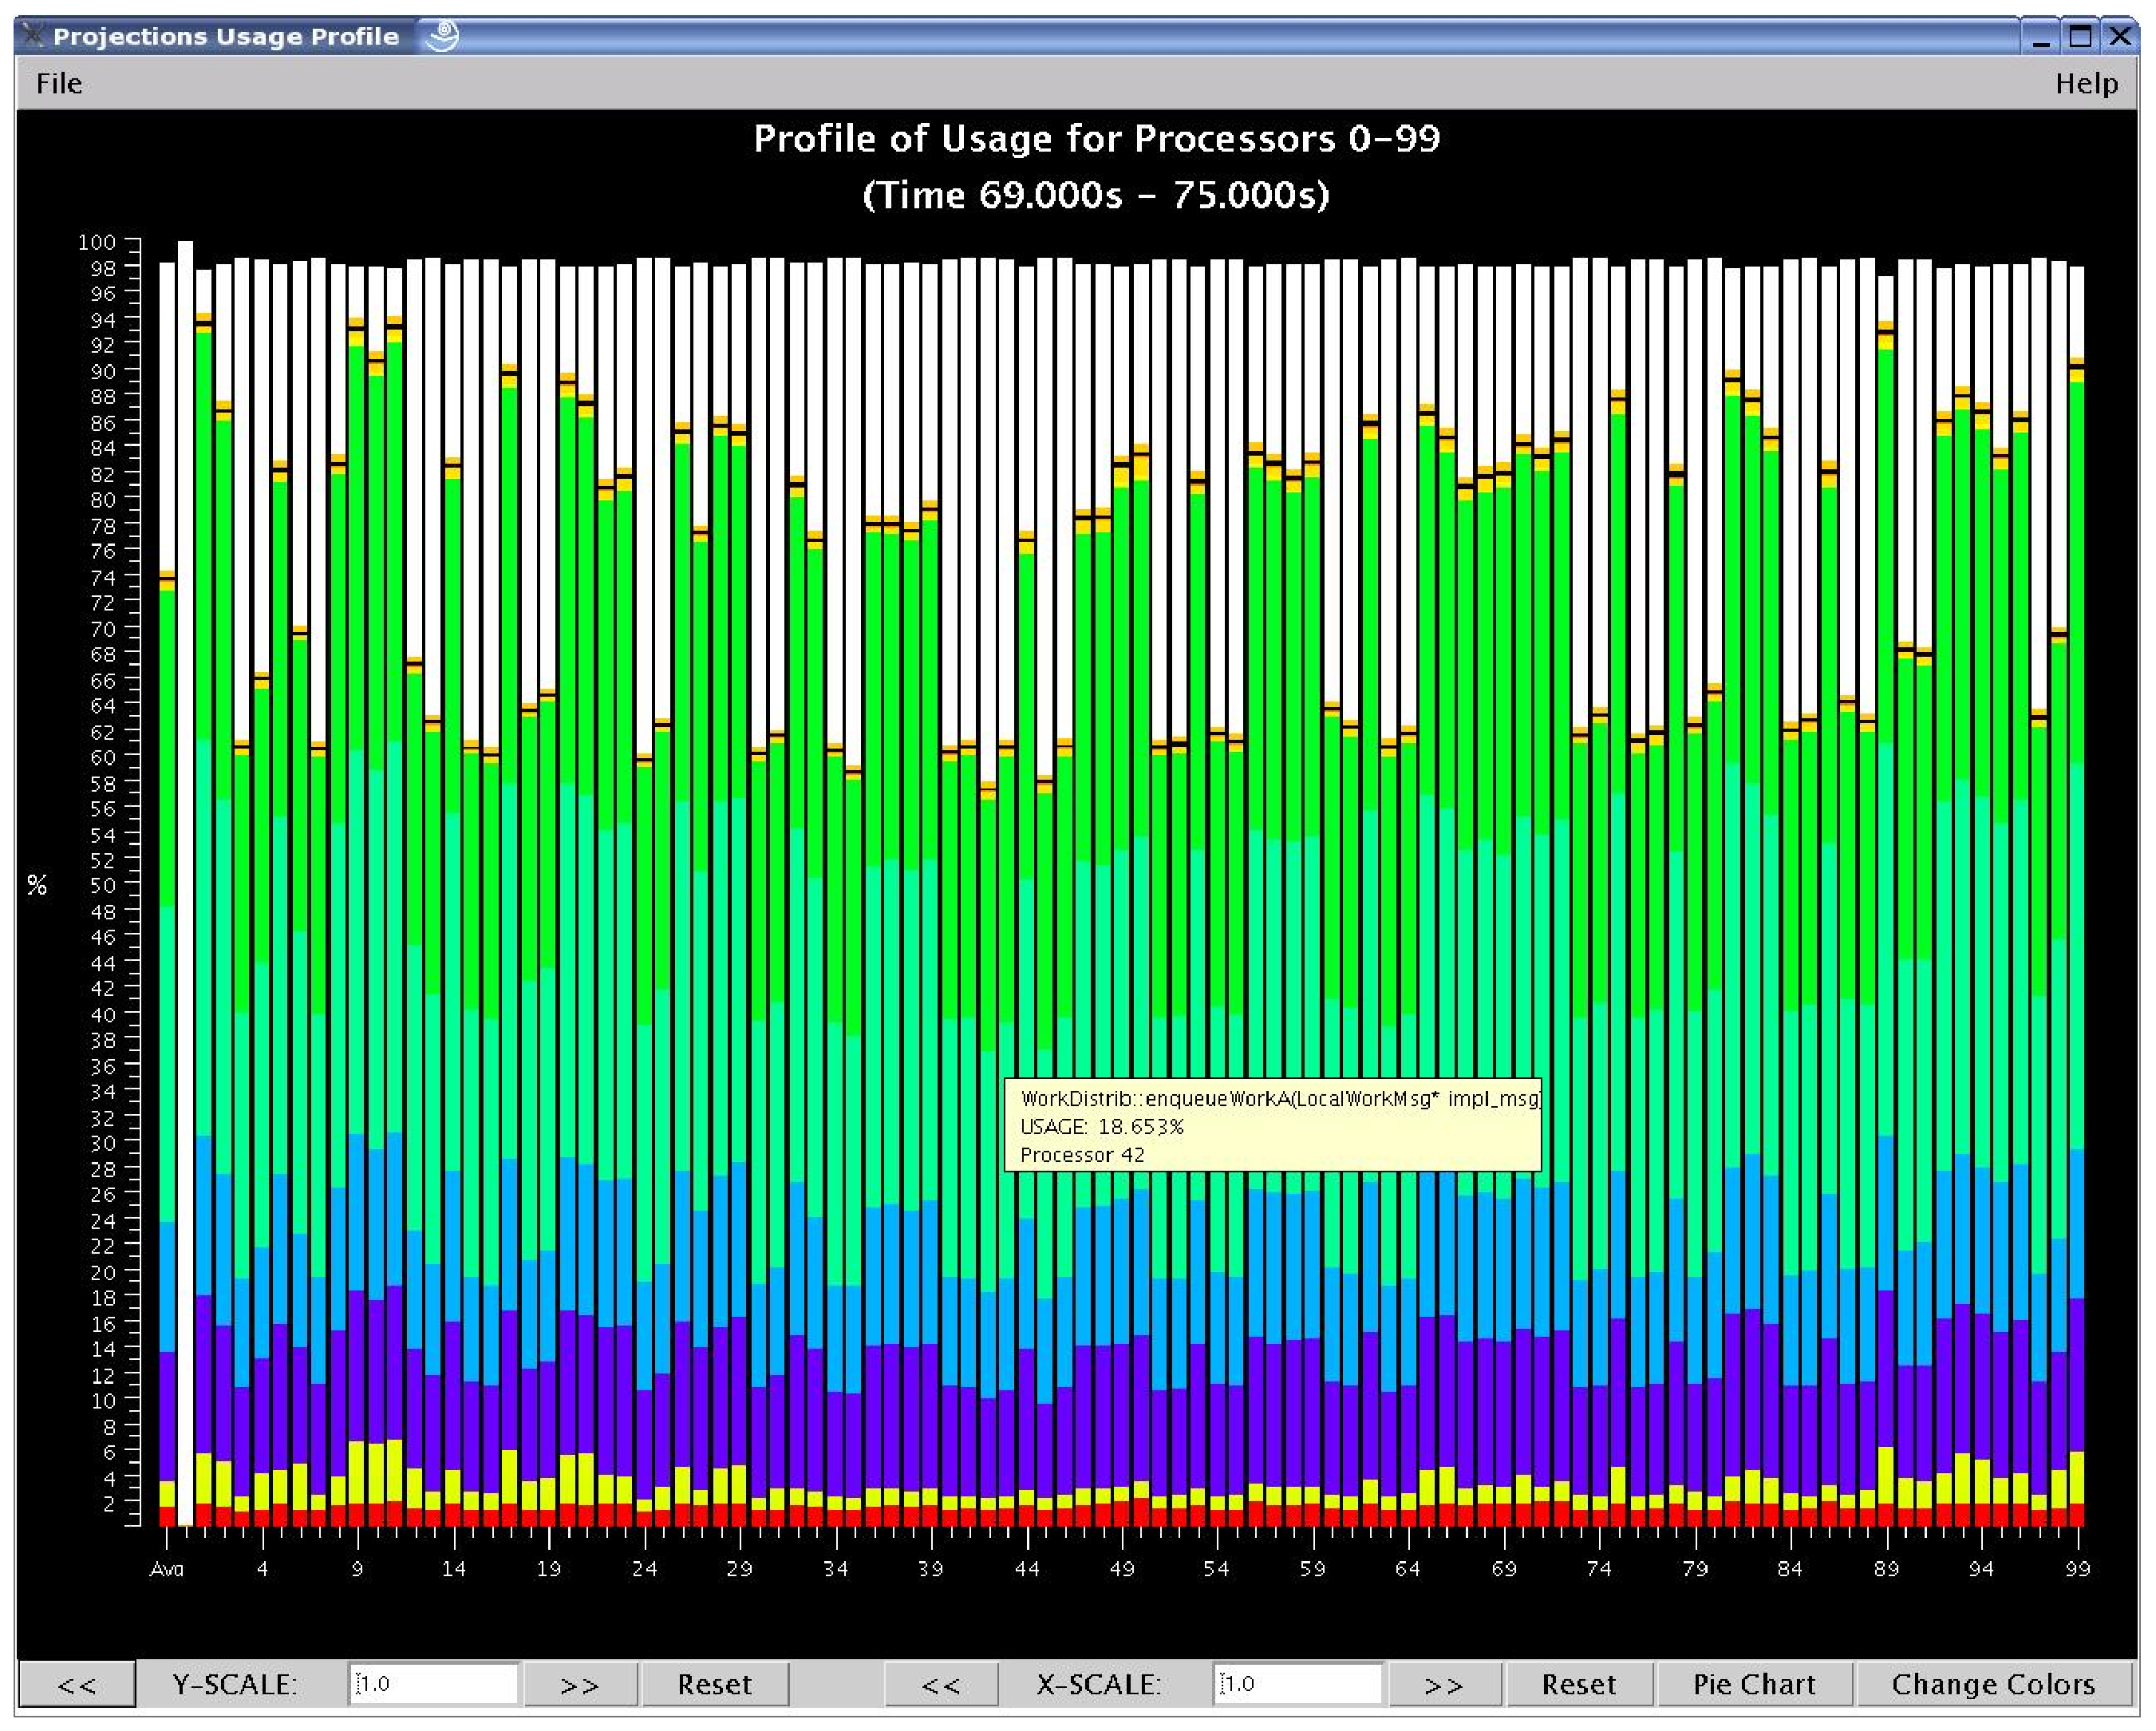
\includegraphics[width=4.0in]{fig/usageprofile}
\caption{Usage Profile}
\label{usage profile}
\end{figure}

The bottom portion of the Usage Profile window lets you adjust the
scales in both the X and Y directions.  The X direction is useful if
you are looking at a large number of processors.  The Y direction is
useful if there are small-percentage items for a processor.

The left side of the display shows a scale from 0\% to 100\%.  The
main part of the display shows the statistics.  Each processor is
represented by a vertical bar.  The top of the bar always shows the
overhead time.  Below that is always (if exists) the idle time and
then the message packing/unpacking times.  The rest of the bar is
ordered from the bottom with the largest percentage items being
closest to the bottom.  If you place the cursor over a portion of the
bar, a pop-up window will appear telling you the name of the item,
what percent of the usage it has, and the processor it is on.

\subsubsection{Communication Histograms}

DESCRIPTION OF COMMUNICATION HISTOGRAM FUNCTIONALITY HERE PLEASE ...

\begin{figure}[htb]
\center
%\epsfig{figure=fig/commhistogram.eps,height=4in}
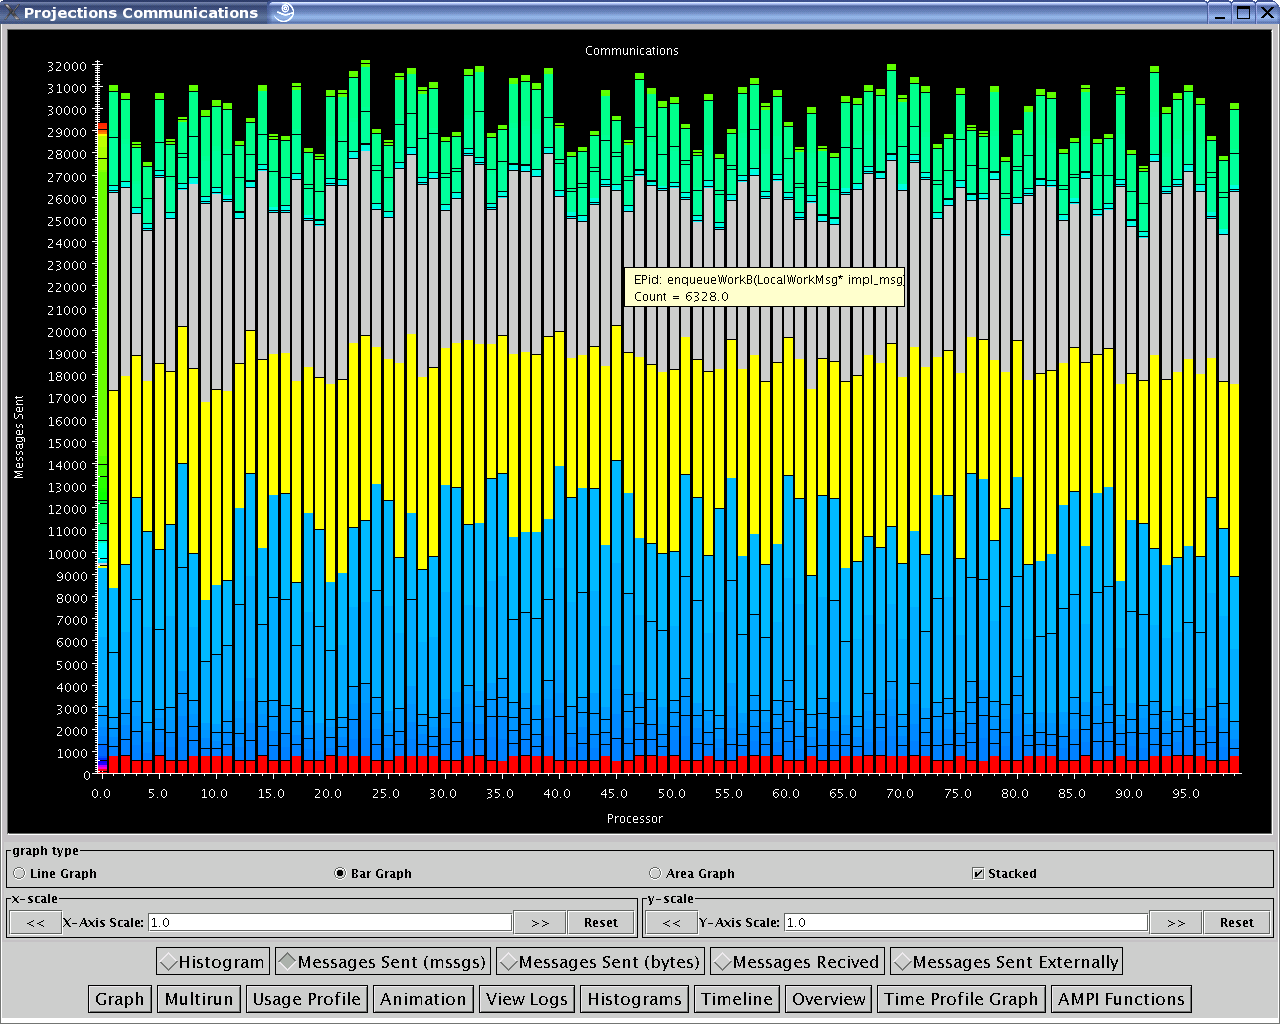
\includegraphics[width=4.0in]{fig/commhistogram}
\caption{Communication Histogram View}
\label{communication histogram}
\end{figure}

\subsubsection{View Log Files}

This window lets you see a translation of a log file from a bunch of
numbers to an English version.  A dialog box asks which processor you
want to look at.  After choosing and pressing OK, the translated
version appears.

Each line has:
\begin{itemize}
\item[-] a line number (starting at 0)
\item[-] the time the event occurred at
\item[-] a description of what happened.
\end{itemize}

\subsubsection{Histograms}

This module allows you to examine the execution time distribution of all your
entry points(EP). It gives a histogram of different number of EP's that have
execution time falling in different time bins.

\begin{figure}[htb]
\center
%\epsfig{figure=fig/histogram.eps,height=4in}
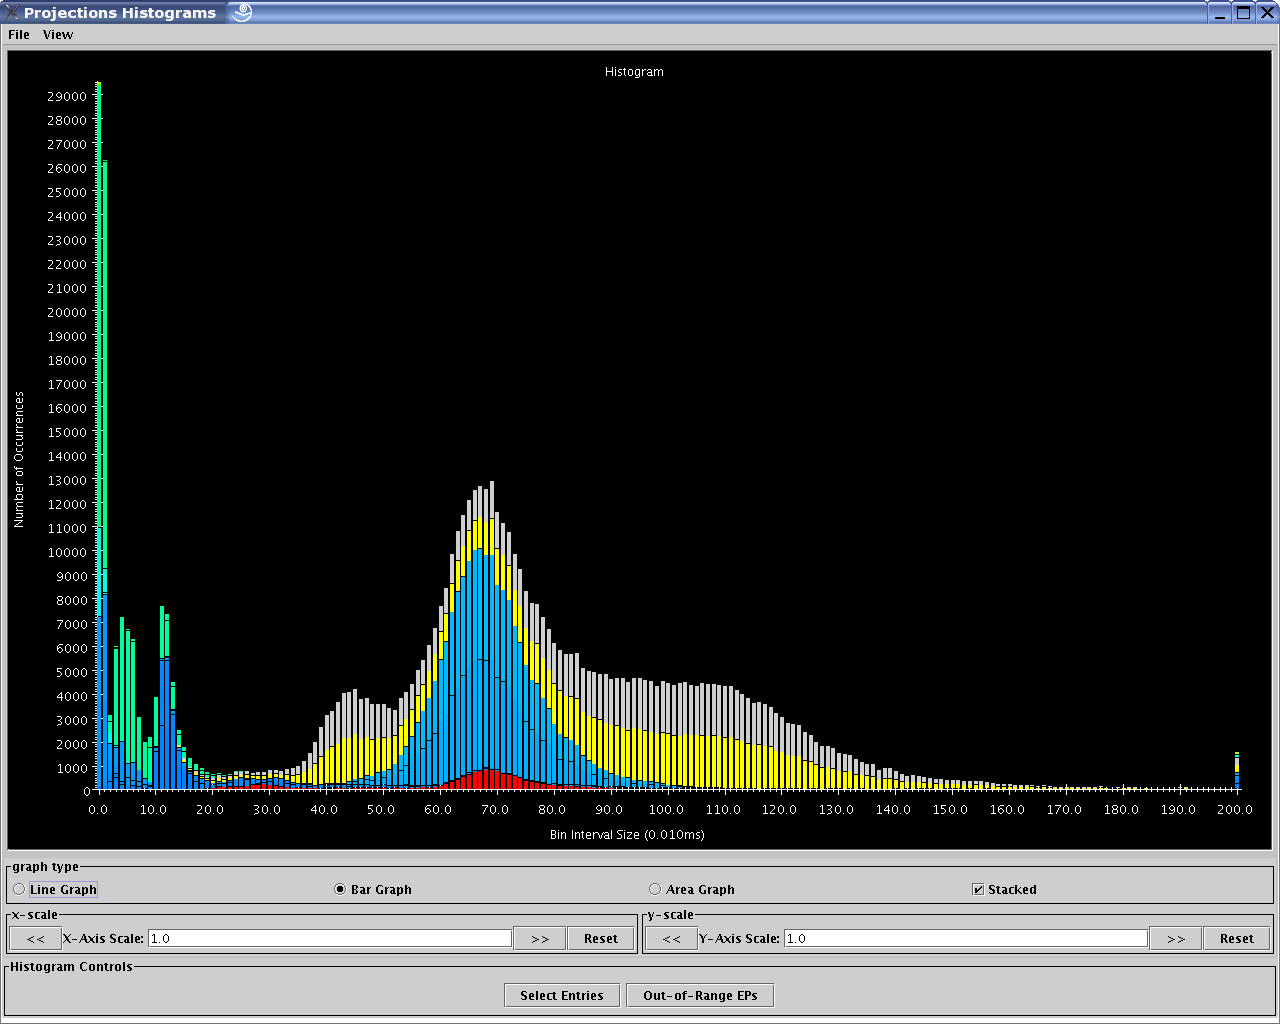
\includegraphics[width=4.0in]{fig/histogram}
\caption{Histogram view}
\label{histogram}
\end{figure}

A dialog allows you to specify the number of bins, the size of each
bin and the minimum bin size you wish to start counting the entry
method by.

The following features are, as of this writing, not implemented. They
will be ready very soon.

The ``Select Entries'' button brings up a color selection and
filtering window that allows you to filter away entry methods from the
count. This offers more control over the analysis (e.g. when you
already know EP 5 takes 20-30ms and you want to know if there
are other entry points also takes 20-30ms).

The ``Out-of-Range EPs'' button brings up a table detailing all the
entry methods that fall into the overflow (last) bin. This list will,
by default, be listed in descending order of time taken by the entry
methods.

\subsubsection{Overview}

Overview gives user an overview of the utilization of all processors
during the execution. 

\begin{figure}[htb]
\center
%\epsfig{figure=fig/overview.eps,height=4in}
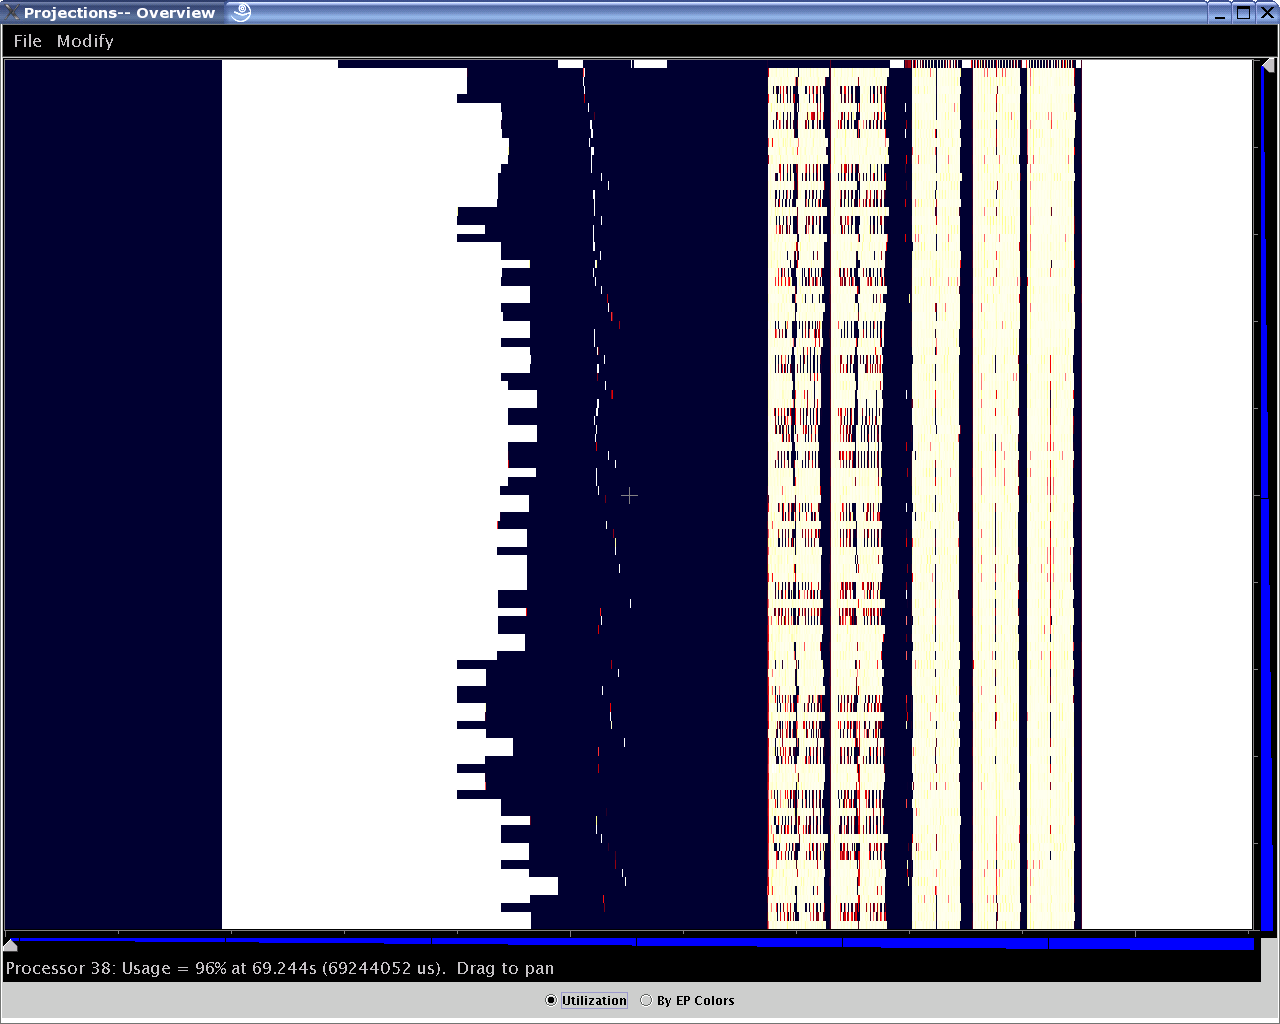
\includegraphics[width=4.0in]{fig/overview}
\caption{Overview}
\label{overview}
\end{figure}

Each processor has a row of colored bars in the display, different
colors indicating different utilization at that time. Moving a mouse
over the graph will invoke a display of the processor usage of the
specific processor at the specific time in the status bar below the
graph. Vertical and horizontal zoom is enabled by two zooming bars to
the right and lower of the graph.

The ``by EP colors'' radio button provides more detail by replacing
the utilization colors with the colors of the most significant entry
method execution time in that time-interval on that processor
represented by the cells. Be warned that this is very likely a major
visualization resource hog.

\subsubsection{Animations}

This window animates the processor usage over a specified range of
time and a specified interval size. 

\begin{figure}[htb]
\center
%\epsfig{figure=fig/animation.eps,height=4in}
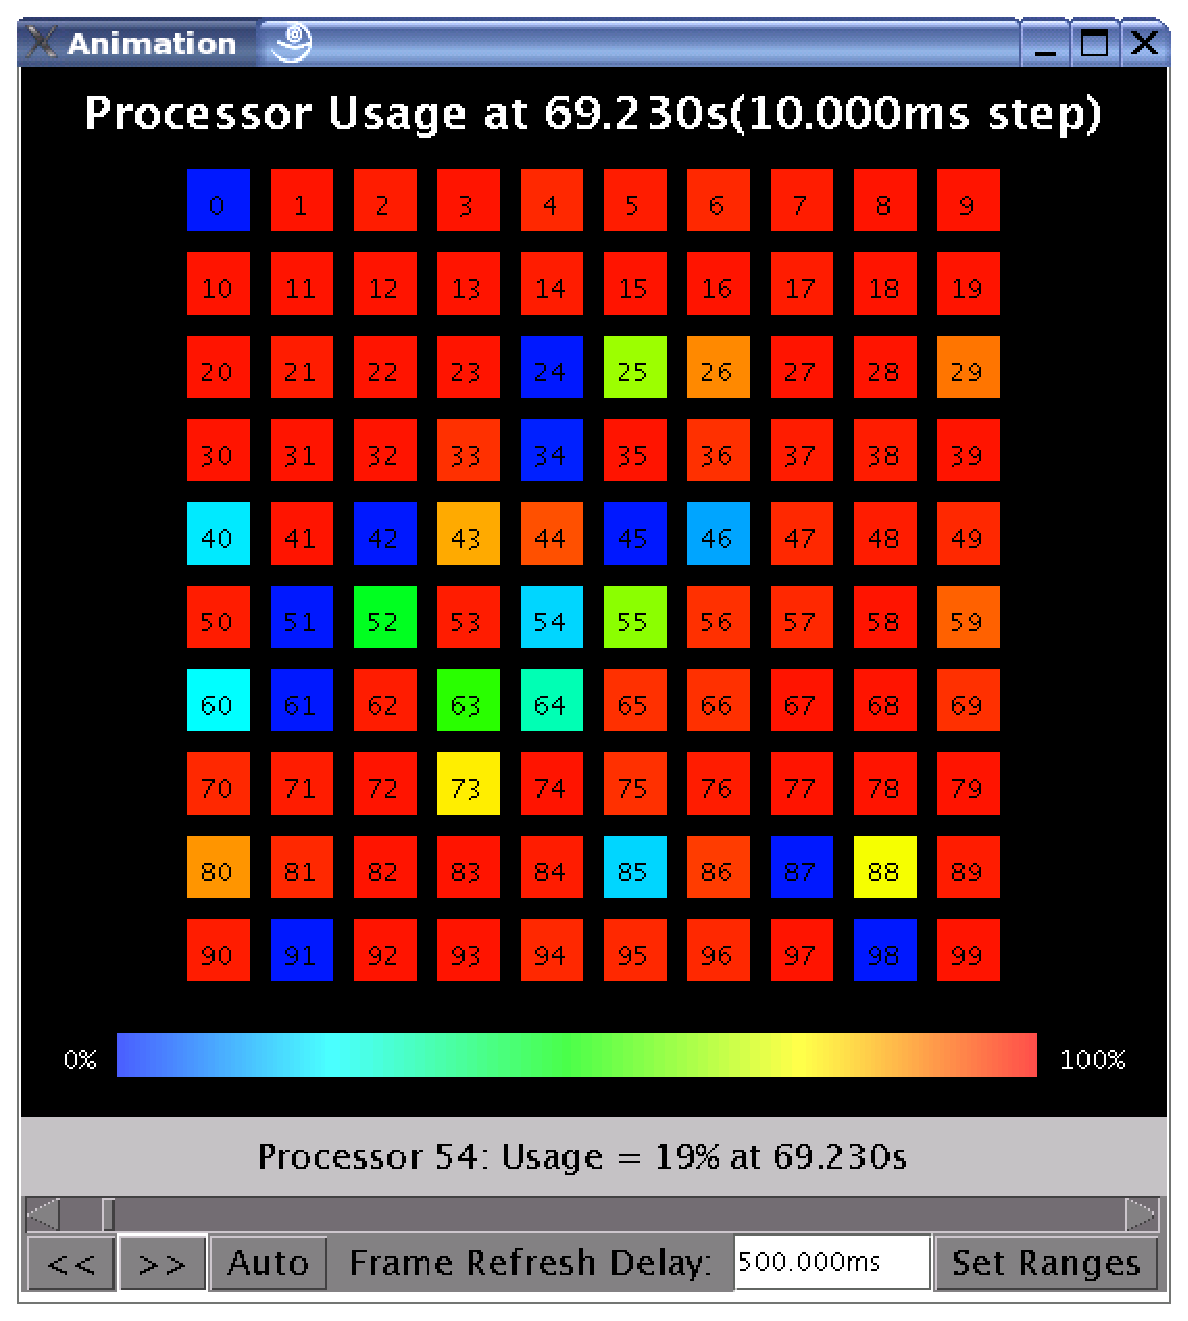
\includegraphics[width=4.0in]{fig/animation}
\caption{Animation View}
\label{animation}
\end{figure}

A dialog is initially displayed to allow you to specify initial time
range, desired processors and the time interval size.

A color temperature bar serves as a legend for displaying different
processor utilizations as the animation progresses.

You may manually update the frames by using the ``<<'' or ``>>''
buttons to visualize the preceding or next frames respectively.

The ``Frame Refresh Delay'' field allows you to select the real time
delay between frames. The ``Auto'' button toggles automatic animation
given the desired refresh rate.

The ``Set Ranges'' button allows you to set new parameters for this
view.

\subsubsection{Time Profile Graph}

DESCRIPTION OF THE TIME PROFILE GRAPH TOOL.

\begin{figure}[htb]
\center
%\epsfig{figure=fig/timeprofile.eps,height=4in}
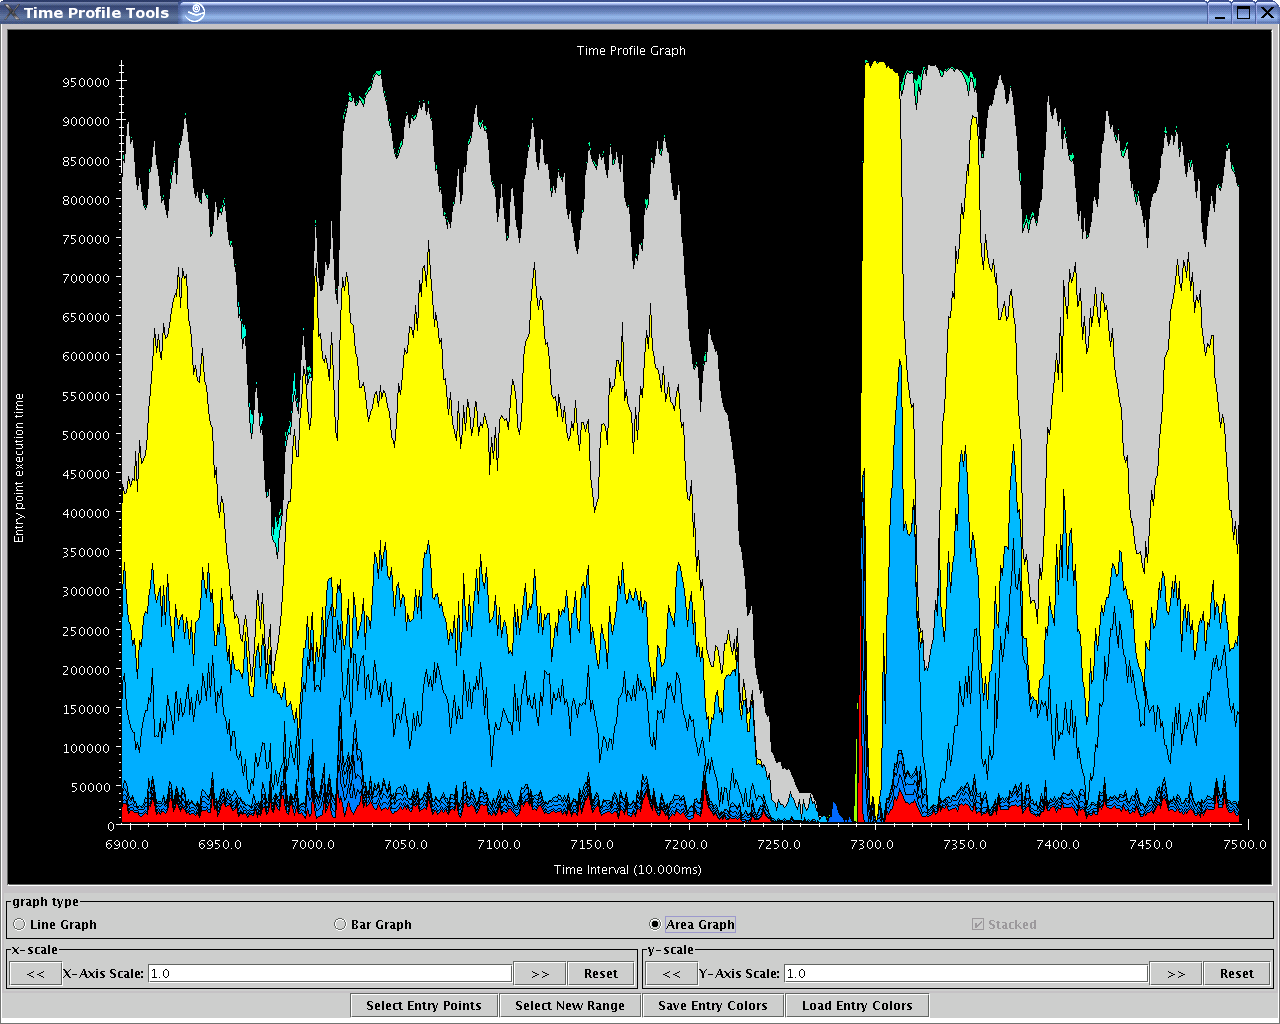
\includegraphics[width=4.0in]{fig/timeprofile}
\caption{Time Profile Graph View}
\label{time profile}
\end{figure}

\subsubsection{Multirun Analysis}

DESCRIPTION OF THE MULTIRUN ANALYSIS TOOL.

\subsubsection{Miscellaneous Features}

DESCRIBE AND SHOW THE USE OF VARIOUS PROJECTIONS DIALOG WINDOWS.

\section{Tutorial: A Performance Analysis Exercise}

DO A TYPICAL PERFORMANCE ANALYSIS EXERCISE, DESCRIBING COMMON THINGS TO
WATCH OUT FOR WHEN USING PROJECTIONS.

\end{document}
